% Copyright (c) 2026 Twin Vector Labs LLC.
% All rights reserved.
\documentclass[11pt]{article}

\usepackage[T1]{fontenc}
\usepackage{lmodern}
\usepackage[margin=1in]{geometry}
\usepackage{amsmath,amssymb,amsthm,mathtools}
\usepackage{booktabs}
\usepackage{enumitem}
\usepackage{xcolor}
\usepackage{microtype}
\usepackage{tikz}
\usetikzlibrary{arrows.meta,positioning,calc}
\usepackage[colorlinks=true,linkcolor=blue!50!black,citecolor=green!40!black,urlcolor=blue!60!black]{hyperref}

% --- operators ---
\DeclareMathOperator{\Tr}{Tr}
\DeclareMathOperator{\vecop}{vec}
\DeclareMathOperator{\rank}{rank}
\DeclareMathOperator{\diag}{diag}
\DeclareMathOperator{\Hom}{Hom}
\DeclareMathOperator{\im}{im}
\DeclareMathOperator{\spn}{span}
\DeclareMathOperator*{\argmin}{arg\,min}
\newcommand{\HH}{\mathcal{H}}
\newcommand{\LL}{\mathcal{L}}
\newcommand{\R}{\mathbb{R}}
\newcommand{\C}{\mathbb{C}}
\newcommand{\Z}{\mathbb{Z}}
\newcommand{\ket}[1]{\lvert #1 \rangle}
\newcommand{\bra}[1]{\langle #1 \rvert}
\newcommand{\braket}[2]{\langle #1 \vert #2 \rangle}
\newcommand{\inner}[2]{\langle #1, #2 \rangle}
\newcommand{\norm}[1]{\lVert #1 \rVert}
\newcommand{\abs}[1]{\lvert #1 \rvert}
\newcommand{\bd}{\partial}
\newcommand{\dd}{\mathrm{d}}
\newcommand{\harm}{\mathcal{H}}              % harmonic space
\newcommand{\gin}{g_{\mathrm{in}}}
\newcommand{\gout}{g_{\mathrm{out}}}
\newcommand{\ZT}{Z_{T}}
\newcommand{\Zdw}{Z_{\mathrm{DW}}}
\newcommand{\Zsp}{Z_{\mathrm{spec}}}
\newcommand{\rU}{r_{U}}
\newcommand{\code}[1]{\texttt{#1}}

\theoremstyle{plain}
\newtheorem{theorem}{Theorem}[section]
\newtheorem{proposition}[theorem]{Proposition}
\newtheorem{lemma}[theorem]{Lemma}
\newtheorem{corollary}[theorem]{Corollary}
\theoremstyle{definition}
\newtheorem{definition}[theorem]{Definition}
\newtheorem{remark}[theorem]{Remark}
\newtheorem{assumption}[theorem]{Assumption}

% honest-caveat callout (matches bulk_synthesis_theory.tex)
\newcommand{\caveat}[1]{\par\noindent\textcolor{red!60!black}{\textbf{Caveat.}}\ #1\par}

\title{\bfseries Transition Amplitudes and Probabilities\\ from Relaxed Cobordisms\\[4pt]
\large Theory, Provenance, and Two Extensions}
\author{Tessera --- cobordism subsystem}
\date{}

\begin{document}
\maketitle

\begin{abstract}
\noindent
We collect, derive from first principles, and critically assess the machinery by which
the Tessera cobordism subsystem reads a \emph{transition amplitude}
$Z(W)=\braket{\psi_A}{U\,\psi_B}$ off a simplicial cobordism $W$ after a relaxation
step. The construction rests on four layers, each of a different epistemic status:
(i) discrete Hodge theory, which makes harmonic $k$-forms the boundary state space
(theorem); (ii) the topology of the carried register, which decides \emph{which} boundary
states a given bulk can transport (theorem); (iii) the Choi--Jamio\l{}kowski map--state
duality, which identifies the operation reading with the pairing (algebraic identity);
and (iv) a TQFT gluing law, under which stacked cobordisms compose and amplitudes
interfere. We derive the exact transport-amplitude identity
$\ZT(q,\alpha)=(T^{-1}q)^\dagger G\,\alpha$ and its deviation law, locate the emergent
gate as $u'=(T^\dagger)^{-1}$, and prove that probability normalization
$\sum_b\abs{Z}^2=1$ is \emph{exactly} the unitarity of $u'$. We then specify two
extensions that are not yet certified: a normalized-probability experiment (Born rule
$+$ coherent composition) and the coupling of the full complex Regge action relaxation to
the amplitude readout. Throughout we separate what is a theorem from what is a numerical
certificate from what is conjectural, and we flag the conformal runaway and the
discretization floor as the load-bearing physical caveats.
\end{abstract}

\tableofcontents
\bigskip

\section{Scope and provenance}
\label{sec:scope}

This document is theory, not a results report. It formalizes the content of two committed
capstone examples and the algebraic oracle they lean on:
\begin{itemize}[nosep]
  \item \code{examples/cobordism/dw\_spectral\_bridge.py} (the v0.4 bridge, \#174): three
        independent readings $\Zdw=\braket{\psi_A}{U\,\psi_B}=\Zsp$ on $\Sigma=T^2$;
  \item \code{examples/cobordism/level1\_value\_reading.py} (\#280/\#284): the anchored
        transport value $\ZT(q,\alpha)$ and its exact deviation law;
  \item \code{include/quantum/ChoiJamiolkowski.h}: the dense map--state duality;
  \item \code{examples/cobordism/stationary\_action\_relaxation.py} (\#340/\#343): the
        $\Phi=\norm{\nabla S}^2+\Gamma\,\rU$ objective.
\end{itemize}
The amplitude bridge uses \emph{spectral} realizability (the Hodge picture), which is
metric-light; the full \emph{stationary-action} relaxation is a separate object, and the
fact that the two are not yet wired together is the central open problem
(\S\ref{sec:backreaction}--\S\ref{sec:experiments}).

\section{The state space: discrete Hodge theory}
\label{sec:hodge}

Let $\Sigma$ be a finite simplicial complex with a metric (edge squared-lengths $\ell$).
On $k$-cochains $C^k=C^k(\Sigma;\C)$ the metric induces the weighted inner product through
the circumcentric dual volumes (the Hodge weights $w_k$),
\begin{equation}
  \inner{a}{b}_k \;=\; \sum_{\sigma\in\Sigma_k} w_k(\sigma)\,\overline{a(\sigma)}\,b(\sigma).
  \label{eq:hodge-inner}
\end{equation}
The coboundary $d_k:C^k\to C^{k+1}$, $(d_k a)(\tau)=\sum_{\sigma\subset\tau}[\sigma:\tau]a(\sigma)$,
has the Hodge adjoint $\delta_k=W_k^{-1}d_k^{\mathsf T}W_{k+1}$ with respect to
\eqref{eq:hodge-inner}, where $W_k=\diag(w_k)$. The Hodge Laplacian is
\begin{equation}
  L_k \;=\; \delta_k d_k + d_{k-1}\delta_{k-1},
\end{equation}
which the code assembles in symmetric form (\code{numpy\_L1}):
\begin{equation}
  L_1^{\mathrm{sym}} = B_1^{\mathsf T}B_1 + B_2 B_2^{\mathsf T},\qquad
  B_1 = d_1 W_1^{-1/2},\quad B_2 = W_1^{1/2}d_2 W_2^{-1/2}.
\end{equation}

\begin{theorem}[Discrete Hodge decomposition]
\label{thm:hodge}
There is an orthogonal decomposition $C^k = \im d_{k-1} \oplus \ker L_k \oplus \im \delta_k$,
and the harmonic space $\harm^k:=\ker L_k$ satisfies $\harm^k \cong H^k(\Sigma;\C)$, so
$\dim\harm^k = b_k$, the $k$-th Betti number.
\end{theorem}

\begin{definition}[Spectral qubit]
The boundary state space is $\HH_\Sigma := \harm^k(\Sigma)$ with the inner product
\eqref{eq:hodge-inner} restricted to it. Harmonic forms \emph{are} states; the Hodge inner
product \emph{is} the quantum inner product.
\end{definition}

For $\Sigma=T^2$, $k=1$: $b_1=2$, so $\HH_{T^2}=\C^2$, spanned by the longitude and meridian
classes.

\begin{remark}[Two distinct state spaces]
The Dijkgraaf--Witten space $\Zdw(\Sigma)=\C[H^1(\Sigma;\Z_2)]=\C^4$ is the \emph{group-algebra}
state space, of dimension $2^{b_1}=4$, not $b_1=2$. It is a strictly larger object than the
spectral qubit; \S\ref{sec:gluing} relates the two via the ``quantized shadow.'' They must not
be conflated.
\end{remark}

\section{Cobordism transport: the carried register}
\label{sec:transport}

Let $W$ be a cobordism with $\bd W = M_0 \sqcup \overline{M_1}$. The inclusions
$\iota_a:M_a\hookrightarrow W$ pull harmonic forms back to the boundary, and the period map
over a chosen basis of hole-cycles $\{c_i\}$ extracts the register coordinates:
\begin{equation}
  \pi_a:\harm^k(W)\to\C^{b},\qquad (\pi_a h)_i = \oint_{c_i\subset M_a} h
       = \sum_{e\in c_i}\pm\,h(e).
  \label{eq:period}
\end{equation}
(For a triangle hole $(a,b,c)$ this is $h(a,b)+h(b,c)-h(a,c)$, the code's \code{\_period}.)

\begin{definition}[Carried class]
A boundary class is \emph{carried} by $W$ iff it lies in the image of the restriction
$H_k(\bd W)\to H_k(W)$.
\end{definition}

\begin{theorem}[Longitude/meridian dichotomy]
\label{thm:dichotomy}
For the solid torus $W=D^2\times S^1$ one has $H_1(W)=\Z\langle\text{longitude}\rangle$, while
the meridian bounds the disk $D^2$ and so maps to $0$ in $H_1(W)$. Hence the longitude is
carried (spectrally realizable, residual $\to 0$) and the meridian is obstructed (its
realizability residual floors).
\end{theorem}

This is pure algebraic topology: the realizability oracle's verdict is computing the rank of
the restriction map, not a numerical accident. The continuous family
$\cos(s)\,\text{long}+\sin(s)\,\text{mer}$ interpolates between the two and the floor lifts
monotonically (the \code{spectral\_boundary\_sweep}).

\begin{definition}[Transport]
\label{def:transport}
For a \emph{graph-like} fill (both ends carry the full register, so $\pi_0,\pi_1$ are
isomorphisms) the period-level transport is the composite
\begin{equation}
  T \;:=\; \pi_1\circ\pi_0^{-1} \;:\; \C^b\to\C^b,
\end{equation}
sending end-0 periods to end-1 periods.
\end{definition}

\begin{center}
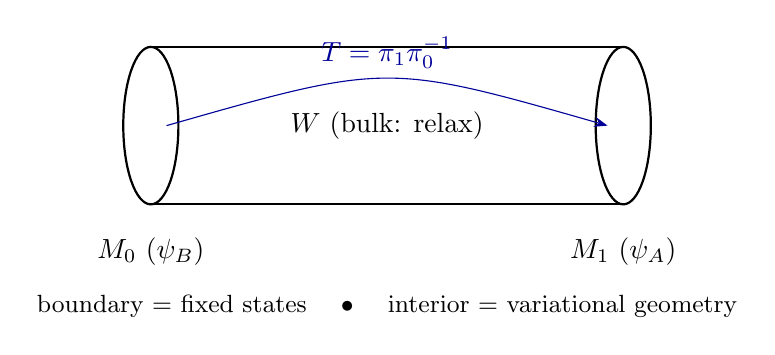
\begin{tikzpicture}[>=Stealth,scale=1.0]
  \draw[thick] (0,-1) ellipse (0.35 and 1);
  \draw[thick] (6,-1) ellipse (0.35 and 1);
  \draw[thick] (0,0) -- (6,0);
  \draw[thick] (0,-2) -- (6,-2);
  \node at (0,-2.6) {$M_0$ ($\psi_B$)};
  \node at (6,-2.6) {$M_1$ ($\psi_A$)};
  \node at (3,-1) {$W$ (bulk: relax)};
  \draw[->,blue!60!black] (0.2,-1) .. controls (3,-0.2) .. (5.8,-1)
     node[midway,above,blue!60!black]{$T=\pi_1\pi_0^{-1}$};
  \node[align=center] at (3,-3.3)
     {\small boundary $=$ fixed states $\quad\bullet\quad$ interior $=$ variational geometry};
\end{tikzpicture}
\end{center}

\section{The chart, the Gram, and the exact amplitude identity}
\label{sec:amplitude}

Use end-0 periods as a coordinate chart on $\harm^k(W)$. Define the two named harmonics
\begin{equation}
  \gin(\alpha) := \pi_0^{-1}(\alpha),\qquad
  \gout(q) := \pi_1^{-1}(q) = \pi_0^{-1}(T^{-1}q) = \gin(T^{-1}q).
  \label{eq:gin-gout}
\end{equation}
The Hodge inner product, expressed in the end-0 chart, is a Hermitian Gram form $\tilde G$,
$\inner{\pi_0^{-1}(x)}{\pi_0^{-1}(y)} = (1/s_1)\,x^\dagger G\,y$, where $G=s_1\tilde G$ is the
\emph{anchor-normalized} Gram and the anchor is fixed by one reference state,
$s_1^{-1}=\inner{\gin(\beta_0)}{\gin(\beta_0)}$. The transport value is the anchored
cross-end pairing,
\begin{equation}
  \ZT(q,\alpha) \;:=\; s_1\,\inner{\gout(q)}{\gin(\alpha)}.
  \label{eq:ZT-def}
\end{equation}

\begin{proposition}[Exact transport amplitude]
\label{prop:ZT}
With the conventions above,
\begin{equation}
  \boxed{\;\ZT(q,\alpha) \;=\; (T^{-1}q)^\dagger\,G\,\alpha\;}
  \label{eq:ZT}
\end{equation}
\end{proposition}
\begin{proof}
Substitute $\gout(q)=\gin(T^{-1}q)$ from \eqref{eq:gin-gout} into \eqref{eq:ZT-def} and use
the Gram identity:
$\ZT = s_1\inner{\gin(T^{-1}q)}{\gin(\alpha)} = s_1\cdot(1/s_1)(T^{-1}q)^\dagger G\,\alpha
= (T^{-1}q)^\dagger G\,\alpha$.
\end{proof}

\begin{definition}[Hand amplitude and the emergent gate]
Let the \emph{hand amplitude} be $\mathrm{amp}(q,\alpha):=(T^{-1}q)^\dagger\alpha
= q^\dagger (T^\dagger)^{-1}\alpha = \braket{q}{u'\,\alpha}$, which \emph{defines} the
emergent gate $u'=(T^\dagger)^{-1}$.
\end{definition}

\begin{corollary}[The deviation law]
\label{cor:devlaw}
Subtracting,
\begin{equation}
  \ZT(q,\alpha) - \braket{q}{u'\,\alpha}
    \;=\; (T^{-1}q)^\dagger\,(G-I)\,\alpha
    \;=\; \tilde w^\dagger\,(G-I)\,\tilde\alpha,
  \label{eq:devlaw}
\end{equation}
with $\tilde w = T^{-1}q$ the end-0 period coordinates of $\gout(q)$ and
$\tilde\alpha$ those of the input. This is exactly the law verified in
\code{level1\_value\_reading.py}.
\end{corollary}

\begin{corollary}[H3: isometric charts]
\label{cor:H3}
If the period chart is Hodge-orthonormal, $G=I$, then $\ZT(q,\alpha)=\braket{q}{u'\,\alpha}$
\emph{identically, for any $T$}. The equivariant ($C_3$-symmetric, no diagonal choices)
prism achieves $G=I$ at machine precision because the end symmetry extends into the bulk;
the staircase prism's order-dependent diagonals break it, giving $\norm{G-I}\sim 10^{-2}$.
\end{corollary}

\begin{remark}[Two independent conditions]
Isometry of the chart ($G=I$, so $\ZT$ reads cleanly) and unitarity of the transport
($T^\dagger T=I$, equivalently $u'=(T^\dagger)^{-1}=T$) are \emph{logically independent}
properties of a fill. A clean unitary quantum amplitude needs both. This separation drives
the two gates of Experiment~A (\S\ref{sec:experiments}).
\end{remark}

\section{The operation reading: Choi--Jamio\l{}kowski}
\label{sec:choi}

The Choi--Jamio\l{}kowski isomorphism bends an operator into a state,
$\vecop(U)=\sum_{ij}U_{ij}\ket{i}\otimes\ket{j}$, with
$\vecop(\ket a\bra b)=a\otimes\overline{b}$ on a rank-one outer product. The central
map--state (Hilbert--Schmidt) duality is an algebraic identity:
\begin{equation}
  \braket{\psi_A}{U\,\psi_B}
    \;=\; \inner{\vecop(U_T)}{\vecop(U)}
    \;=\; \Tr\!\big(U_T^\dagger U\big)
    \;=\; \sum_{ij}\overline{\psi_{A,i}}\,U_{ij}\,\psi_{B,j},
  \qquad U_T=\ket{\psi_A}\bra{\psi_B}.
  \label{eq:choi}
\end{equation}
Because \eqref{eq:choi} holds with no reference to geometry, the ``operation'' reading is a
trustworthy oracle against which the spectral reading is checked. In
\code{dw\_spectral\_bridge.py} the three readings
\begin{equation}
  \Zdw(W)\;=\;\braket{\psi_A}{U\,\psi_B}\;=\;\Zsp
\end{equation}
agree to $10^{-7}$ on longitude-aligned states, each cross-checked against an independent
\code{numpy} reimplementation (a GF(2) state sum, a direct \code{vdot}, and a $\ker L_1$
projection).

\section{Gluing and coherent composition}
\label{sec:gluing}

The framework is a discrete Atiyah TQFT: a closed $(d{-}1)$-manifold $\Sigma$ gets a space
$\HH_\Sigma$, a cobordism $W:\Sigma_0\to\Sigma_1$ gets a linear map $Z(W)$, and
\begin{equation}
  W=W_2\circ_{\Sigma_1}W_1 \;\Rightarrow\; Z(W)=Z(W_2)\,Z(W_1),\qquad
  \HH_{\Sigma\sqcup\Sigma'}=\HH_\Sigma\otimes\HH_{\Sigma'},\qquad Z(\varnothing)=\C.
  \label{eq:gluing}
\end{equation}
Stacked fills compose (verified to $10^{-9}$). Consequently amplitudes compose
\emph{coherently} --- the sum over intermediate states happens \emph{before} the modulus:
\begin{align}
  Z(b,a) &= \bra{b}Z(W_2)Z(W_1)\ket{a} = \sum_m Z_2(b,m)\,Z_1(m,a), \label{eq:cohere}\\
  P(b|a) &= \Big|\textstyle\sum_m Z_2(b,m)Z_1(m,a)\Big|^2
          \;\neq\; \sum_m \abs{Z_2(b,m)}^2\abs{Z_1(m,a)}^2. \label{eq:interfere}
\end{align}
The difference between \eqref{eq:interfere} and the classical (Markov) right-hand side is the
interference cross-term $2\,\mathrm{Re}\sum_{m\neq m'}\!Z_2(b,m)Z_1(m,a)\overline{Z_2(b,m')Z_1(m',a)}$:
the operational signature of a genuine quantum amplitude.

\begin{remark}[The quantized shadow]
The Dijkgraaf--Witten invariant is the state sum
$\Zdw(W)=\sum_{\phi\in\,\text{flat }\Z_2\text{-conn.}}\ \prod_{\text{simplices}}\omega(\phi)$.
For trivial or sign cocycle the values are integer-quantized, so $\im(\Zdw)\subset\Hom(\HH)$ is a
\emph{discrete lattice}. The spectral $Z$ is a continuum (it realizes the longitude and a
neighborhood). Hence $\Zdw=\Zsp$ only at the lattice points; a generic $U$ leaves it
continuously, the gap opening as $U$ departs the discrete DW image. The topological theory is
the integer skeleton of the spectral one.
\end{remark}

\section{Born normalization is exactly unitarity}
\label{sec:born}

\begin{proposition}[Normalization $\Leftrightarrow$ unitarity]
\label{prop:born}
Let $\{b_k\}$ be an orthonormal basis of the output state space, so
$\sum_k\ket{b_k}\bra{b_k}=I$. On an isometric fill ($G=I$, so
$\ZT(b_k,\alpha)=\braket{b_k}{u'\,\alpha}$),
\begin{equation}
  \sum_k P(k|\alpha) = \sum_k \abs{\braket{b_k}{u'\,\alpha}}^2
    = (u'\alpha)^\dagger\Big(\sum_k\ket{b_k}\bra{b_k}\Big)(u'\alpha)
    = \bra{\alpha}u'^\dagger u'\ket{\alpha}.
  \label{eq:born-sum}
\end{equation}
Therefore $\sum_k P(k|\alpha)=\norm{\alpha}^2$ for all $\alpha$ \emph{iff} $u'^\dagger u'=I$,
i.e.\ iff the emergent gate is unitary. Equivalently, since $u'=(T^\dagger)^{-1}$, iff
$T^\dagger T=I$.
\end{proposition}

So probability conservation is not an extra postulate to be imposed --- it is a \emph{theorem
conditioned on a unitarity certificate}. The two hypotheses $\{G=I,\ T^\dagger T=I\}$ are the
complete set; verify them and the Born rule follows. When $G\neq I$ the correct sum is
$\bra{\alpha}u'^\dagger G\,u'\ket{\alpha}$, and \eqref{eq:devlaw} accounts for the deficit
exactly: a non-conserving ``probability'' is then a \emph{measured chart artifact}, not a
hidden leak.

\section{The action and backreaction}
\label{sec:backreaction}

Geometry enters through the weights. The Lorentzian (Sorkin) Regge action is
\begin{equation}
  S(\ell) = \sum_{\text{hinges }h} A_h(\ell)\,\varepsilon_h(\ell)\ \in\ \C,
  \label{eq:regge}
\end{equation}
with $A_h$ the codimension-2 hinge volume and $\varepsilon_h$ the deficit angle, which is
\emph{complex} in Lorentzian signature (spacelike hinges contribute boosts via $\operatorname{acosh}$,
hence imaginary parts). Since the Hodge weights $w_k(\ell)$ are dual volumes, every downstream
object is a functional of $\ell$:
\begin{equation}
  \ell \ \longrightarrow\ L_k(\ell)\ \longrightarrow\ \harm^k(\ell)
       \ \longrightarrow\ T(\ell),\,G(\ell)\ \longrightarrow\ u'(\ell),\,\ZT(\ell).
\end{equation}

\begin{proposition}[How relaxation moves the amplitude]
\label{prop:perturb}
For $L_k(\ell)h=0$ a metric perturbation $\delta\ell$ moves the harmonic by degenerate
first-order perturbation theory,
\begin{equation}
  \delta h = -\,L_k^{+}\,(\delta L_k)\,h, \qquad
  \delta\ZT = s_1\big(\inner{\delta\gout}{\gin}+\inner{\gout}{\delta\gin}\big)
              + (\delta s_1)\inner{\gout}{\gin},
  \label{eq:perturb}
\end{equation}
where $L_k^{+}$ is the Moore--Penrose pseudoinverse on $\im L_k$. Thus $\dd\ZT/\dd\Gamma$ is
computable and is the backreaction signal.
\end{proposition}

The relaxation objective is
\begin{equation}
  \Phi(\ell) = \norm{\nabla S(\ell)}^2 + \Gamma\,\rU(\ell),
  \label{eq:Phi}
\end{equation}
each term load-bearing:
\begin{itemize}[nosep]
  \item $\norm{\nabla S}^2$ drives $\delta S=0$ --- one \emph{extremizes}, never minimizes.
        The bare action is unbounded below (the conformal mode $g\mapsto e^{2\varphi}g$ has a
        wrong-sign kinetic term, hence a runaway), so the stationary point is the target. One
        keeps $\im S$: minimize $\sum\abs{\bd S}^2$, not $\sum(\bd\,\mathrm{Re}\,S)^2$, because
        the imaginary part fixes the overall scale the real part leaves loose.
  \item $\rU=\code{residualForPeriods}$ is the \emph{register fidelity},
        $\rU=\norm{\text{periods}(\text{relaxed harmonic})-\text{target}}$. It is the
        Lagrange-type penalty enforcing $\bd W=(\text{prepared states})$ \emph{under}
        relaxation: the geometry may evolve only while the boundary state stays carried. This
        is the cobordism evolution rule made into an objective.
\end{itemize}

\caveat{Do not sidestep the conformal runaway. The mass that regulates the runaway to a
convergent interior minimum \emph{is} the backreaction physics: no linearizing,
boundary-pinning, or freezing of the matter field, and no swapping the energy functional.}

\begin{remark}[The deep open question]
Does $u'(\ell^\star)$ stay unitary after action relaxation? Relaxation generically breaks the
equivariance that gave $G=I$, so $G(\ell^\star)\neq I$ and possibly
$u'(\ell^\star)^\dagger u'(\ell^\star)\neq I$. By Proposition~\ref{prop:born} that would be
\emph{backreaction-induced apparent non-unitarity} --- probability flowing from the register
into the geometry. Whether the stationary condition $\delta S=0$ \emph{protects} unitarity (a
discrete analogue of unitarity from a real action / reflection positivity) or breaks it is
exactly what Experiment~B would measure. Either answer is a result.
\end{remark}

\section{Two extensions to certify}
\label{sec:experiments}

\paragraph{Experiment A --- normalized transition probabilities.}
Substrate: an \emph{isometric} graph-like transport fill (\code{CellsFill} on the equivariant
$C_3$ prism), where both end blocks $P_0,P_1$ are full rank so the whole register is carried.
\begin{enumerate}[nosep]
  \item Read $u'=\code{emergent\_gate()}$; confirm $\norm{G-I}<10^{-9}$ (chart isometric).
  \item \textbf{Unitarity gate} (the normalization certificate): $\norm{u'^\dagger u'-I}<10^{-9}$.
  \item For random unit inputs $\alpha$, verify $\sum_k\abs{\ZT(b_k,\alpha)}^2=1$ to $10^{-9}$
        (Proposition~\ref{prop:born}).
  \item \textbf{Born $=$ hand}: $\abs{\ZT(b_k,\alpha)}^2=\abs{\braket{b_k}{u'\,\alpha}}^2$.
  \item \textbf{Coherent vs.\ classical}: confirm $P$ obeys \eqref{eq:interfere}, not the Markov
        sum --- the interference cross-term is nonzero (the quantum discriminator).
  \item \textbf{Negative control}: on an anisotropic fill, $\sum_k P\neq 1$ and the deficit equals
        the $(G-I)$ correction of \eqref{eq:devlaw} --- leakage named, not hidden.
\end{enumerate}

\paragraph{Experiment B --- action-coupled amplitude readout.}
Substrate: a transport fill (not a merge --- merge operator readout is deferred, \#376/\#380),
boundary edges pinned to encode $\psi_A,\psi_B$, interior squared lengths variational.
\begin{enumerate}[nosep]
  \item Relax $\Phi(\ell)=\norm{\nabla S}^2+\Gamma\,\rU$ (reuse \code{StationaryActionRelaxation};
        keep $\im S$).
  \item At $\ell^\star$, rebuild $\harm^1(\ell^\star)$, recompute $\gin,\gout,s_1$ and read
        $\ZT(q,\alpha;\ell^\star)$ via Proposition~\ref{prop:perturb}.
  \item \textbf{Reduction}: $\Gamma\to0$, uniform start $\Rightarrow \ZT(\ell^\star)=\ZT(\text{uniform})$.
  \item \textbf{Stationarity}: $\norm{\nabla S}^2(\ell^\star)$ at its intrinsic floor;
        \textbf{register survived}: $\rU(\ell^\star)<\text{tol}$.
  \item \textbf{Backreaction signal}: sweep $\Gamma$; record the continuous shift of
        $\ZT(\ell^\star)$ off the flat value.
  \item \textbf{Unitarity under backreaction}: test $u'(\ell^\star)^\dagger u'(\ell^\star)=I$, with
        any breakage $(G-I)$-accounted.
\end{enumerate}
Sequencing: A before B. A certifies the probability machinery on a clean substrate; B then asks
whether unitarity survives action relaxation. Doing B first means debugging the relaxation and
the Born normalization simultaneously.

\section{Epistemic ledger}
\label{sec:ledger}

\begin{center}
\renewcommand{\arraystretch}{1.25}
\begin{tabular}{@{}p{0.50\textwidth} l@{}}
\toprule
\textbf{Statement} & \textbf{Status} \\
\midrule
$\harm^k(\Sigma)\cong H^k(\Sigma;\C)$; states are harmonic forms (Thm.~\ref{thm:hodge}) & theorem \\
Longitude carried / meridian obstructed (Thm.~\ref{thm:dichotomy}) & theorem (topology) \\
$\ZT=(T^{-1}q)^\dagger G\alpha$ and the deviation law (Prop.~\ref{prop:ZT}, Cor.~\ref{cor:devlaw}) & theorem (derived here) \\
H3: $\ZT=\braket{q}{u'\alpha}$ when $G=I$ (Cor.~\ref{cor:H3}) & theorem; verified $10^{-9}$ \\
Choi map--state identity \eqref{eq:choi} & algebraic identity \\
TQFT gluing / coherent composition \eqref{eq:gluing}--\eqref{eq:interfere} & theorem; composition verified $10^{-9}$ \\
$\Zdw=\braket{\psi_A}{U\psi_B}=\Zsp$ on the DW-representable set & verified $10^{-7}$; \emph{discrete} set only \\
$\sum_k P=1 \Leftrightarrow u'$ unitary (Prop.~\ref{prop:born}) & theorem, \emph{conditional} on the certificate \\
$u'$ \emph{is} unitary on the equivariant fill (Exp.~A, step 2) & \textbf{not yet certified} \\
Coherent (non-Markov) composition of $P$ (Exp.~A, step 5) & \textbf{not yet certified} \\
$\ZT$ read from the action-relaxed $\ell^\star$ (Exp.~B) & \textbf{bridge does not yet exist} \\
$\delta S=0$ protects unitarity under backreaction & \textbf{conjectural} \\
\bottomrule
\end{tabular}
\end{center}

\medskip
\noindent
The solid foundation is \S\ref{sec:hodge}--\S\ref{sec:gluing} (theorems and algebraic
identities). Proposition~\ref{prop:born} is a theorem \emph{conditional on} a certificate that
has not been run. The backreaction coupling of \S\ref{sec:backreaction} is mechanically sound
but physically untested. The two load-bearing physical caveats are the conformal runaway (the
regulator is the physics, not a convenience) and the intrinsic discretization floor
($\sim 4\times10^{-2}$ intertwine residual on non-equivariant metrics), which a
symmetry-invariant metric does not remove.

\end{document}
